\documentclass{experimentreport}

\input{listing_style.tex}

%========================
% Basic Information
%========================

\setcoursename{Intelligence Leading the Frontier, Computing Shaping the Future}
\setreportname{HIT Code Review Research Experiment Report}

\setexperimenttitle{Improving Code Review for Code Generated by Large Models}

\setstudentname{Ulugbek Khamidov, Komil Tokhirov}
\setdepartment{HITCodeReviewResearch}
\setstudentid{2026140348, 2026140354}

\setcourseteacher{Liu Jiakun}
\setinstructor{Liu Jiakun}

\setlablocation{HIT First Campus}
\setlabtime{2024-06-11 14:00-17:00}

\begin{document}

\makereporthead

%========================
% Experiment Objectives
%========================

\experimentpurpose{
- Understood the primary reasons for performance variation of code review on AI-generated code.
- Mastered various methods for constructing code context and their impact on code review tasks.
- Mastered prompt engineering techniques to optimize code review performance.
- Designed prompts suitable for AI-generated code.
- Analyzed the impact of different prompt and context combinations on merge prediction and review comment generation.
- Proposed improvement strategies for code review targeting AI-generated code.
}

%========================
% Experiment Content
%========================

\experimentcontent{
- Loaded AI-generated code dataset (PRs flagged with has\_ai\_code = True).
- Constructed 5 context types with increasing information:
  - C1\_Diff\_Only: Code diff only
  - C2\_Diff\_PR\_Description: Diff + PR title + body + author + commit messages
  - C3\_Diff\_Repo\_Metrics: Diff + code metrics (changed files, additions, deletions, labels)
  - C4\_Diff\_Review\_History: Diff + historical reviews and inline comments
  - C5\_Full\_SE\_Context: Complete context (all of the above combined)
- Designed 4 prompt optimization strategies:
  - P1\_RoleBased: Acting as a Senior Staff Software Engineer
  - P2\_FewShot: In-context learning with examples
  - P3\_ChainOfThought: Step-by-step systematic analysis
  - P4\_SelfReflection: Two-phase analysis with self-critique
- Invoked LLM (Qwen via Ollama) on 21 AI-generated PRs across 5 contexts and 4 prompts (420 evaluations).
- Evaluated using accuracy, precision, recall, F1, and inference latency.
- Compared results against Experiment 3 (human-written code) baseline.
}

%========================
% Experimental Results
%========================

\experimentresult{
We evaluated 21 AI-generated PRs across 5 context types and 4 prompt designs (420 total evaluations).

Overall Performance:
- Accuracy: 49.1\%
- Precision: 42.5\%
- Recall: 53.9\%
- F1-Score: 47.6\%
- Avg Inference Latency: 7.06 seconds

Performance by Context Type:
Context                   Accuracy   F1-Score   Recall
C1\_Diff\_Only            53.6\%     31.6\%     25.0\%
C2\_Diff\_PR\_Description 41.7\%     52.4\%     75.0\%
C3\_Diff\_Repo\_Metrics   51.2\%     51.8\%     61.1\%
C4\_Diff\_Review\_History 52.4\%     33.3\%     27.8\%
C5\_Full\_SE\_Context     46.4\%     56.3\%     80.6\%

Best context: C5\_Full\_SE\_Context (56.3\% F1, 80.6\% recall)

Performance by Prompt Type:
Prompt              Accuracy   F1-Score   Recall
P1\_RoleBased      54.3\%     27.3\%     20.0\%
P2\_FewShot        41.0\%     56.3\%     88.9\%
P3\_ChainOfThought 50.5\%     50.0\%     57.8\%
P4\_SelfReflection 50.5\%     45.8\%     48.9\%

Best prompt: P2\_FewShot (56.3\% F1, 88.9\% recall)

Best combination: C5\_Full\_SE\_Context + P4\_SelfReflection (F1 = 64.3\%)

\begin{figure}[h]
\centering
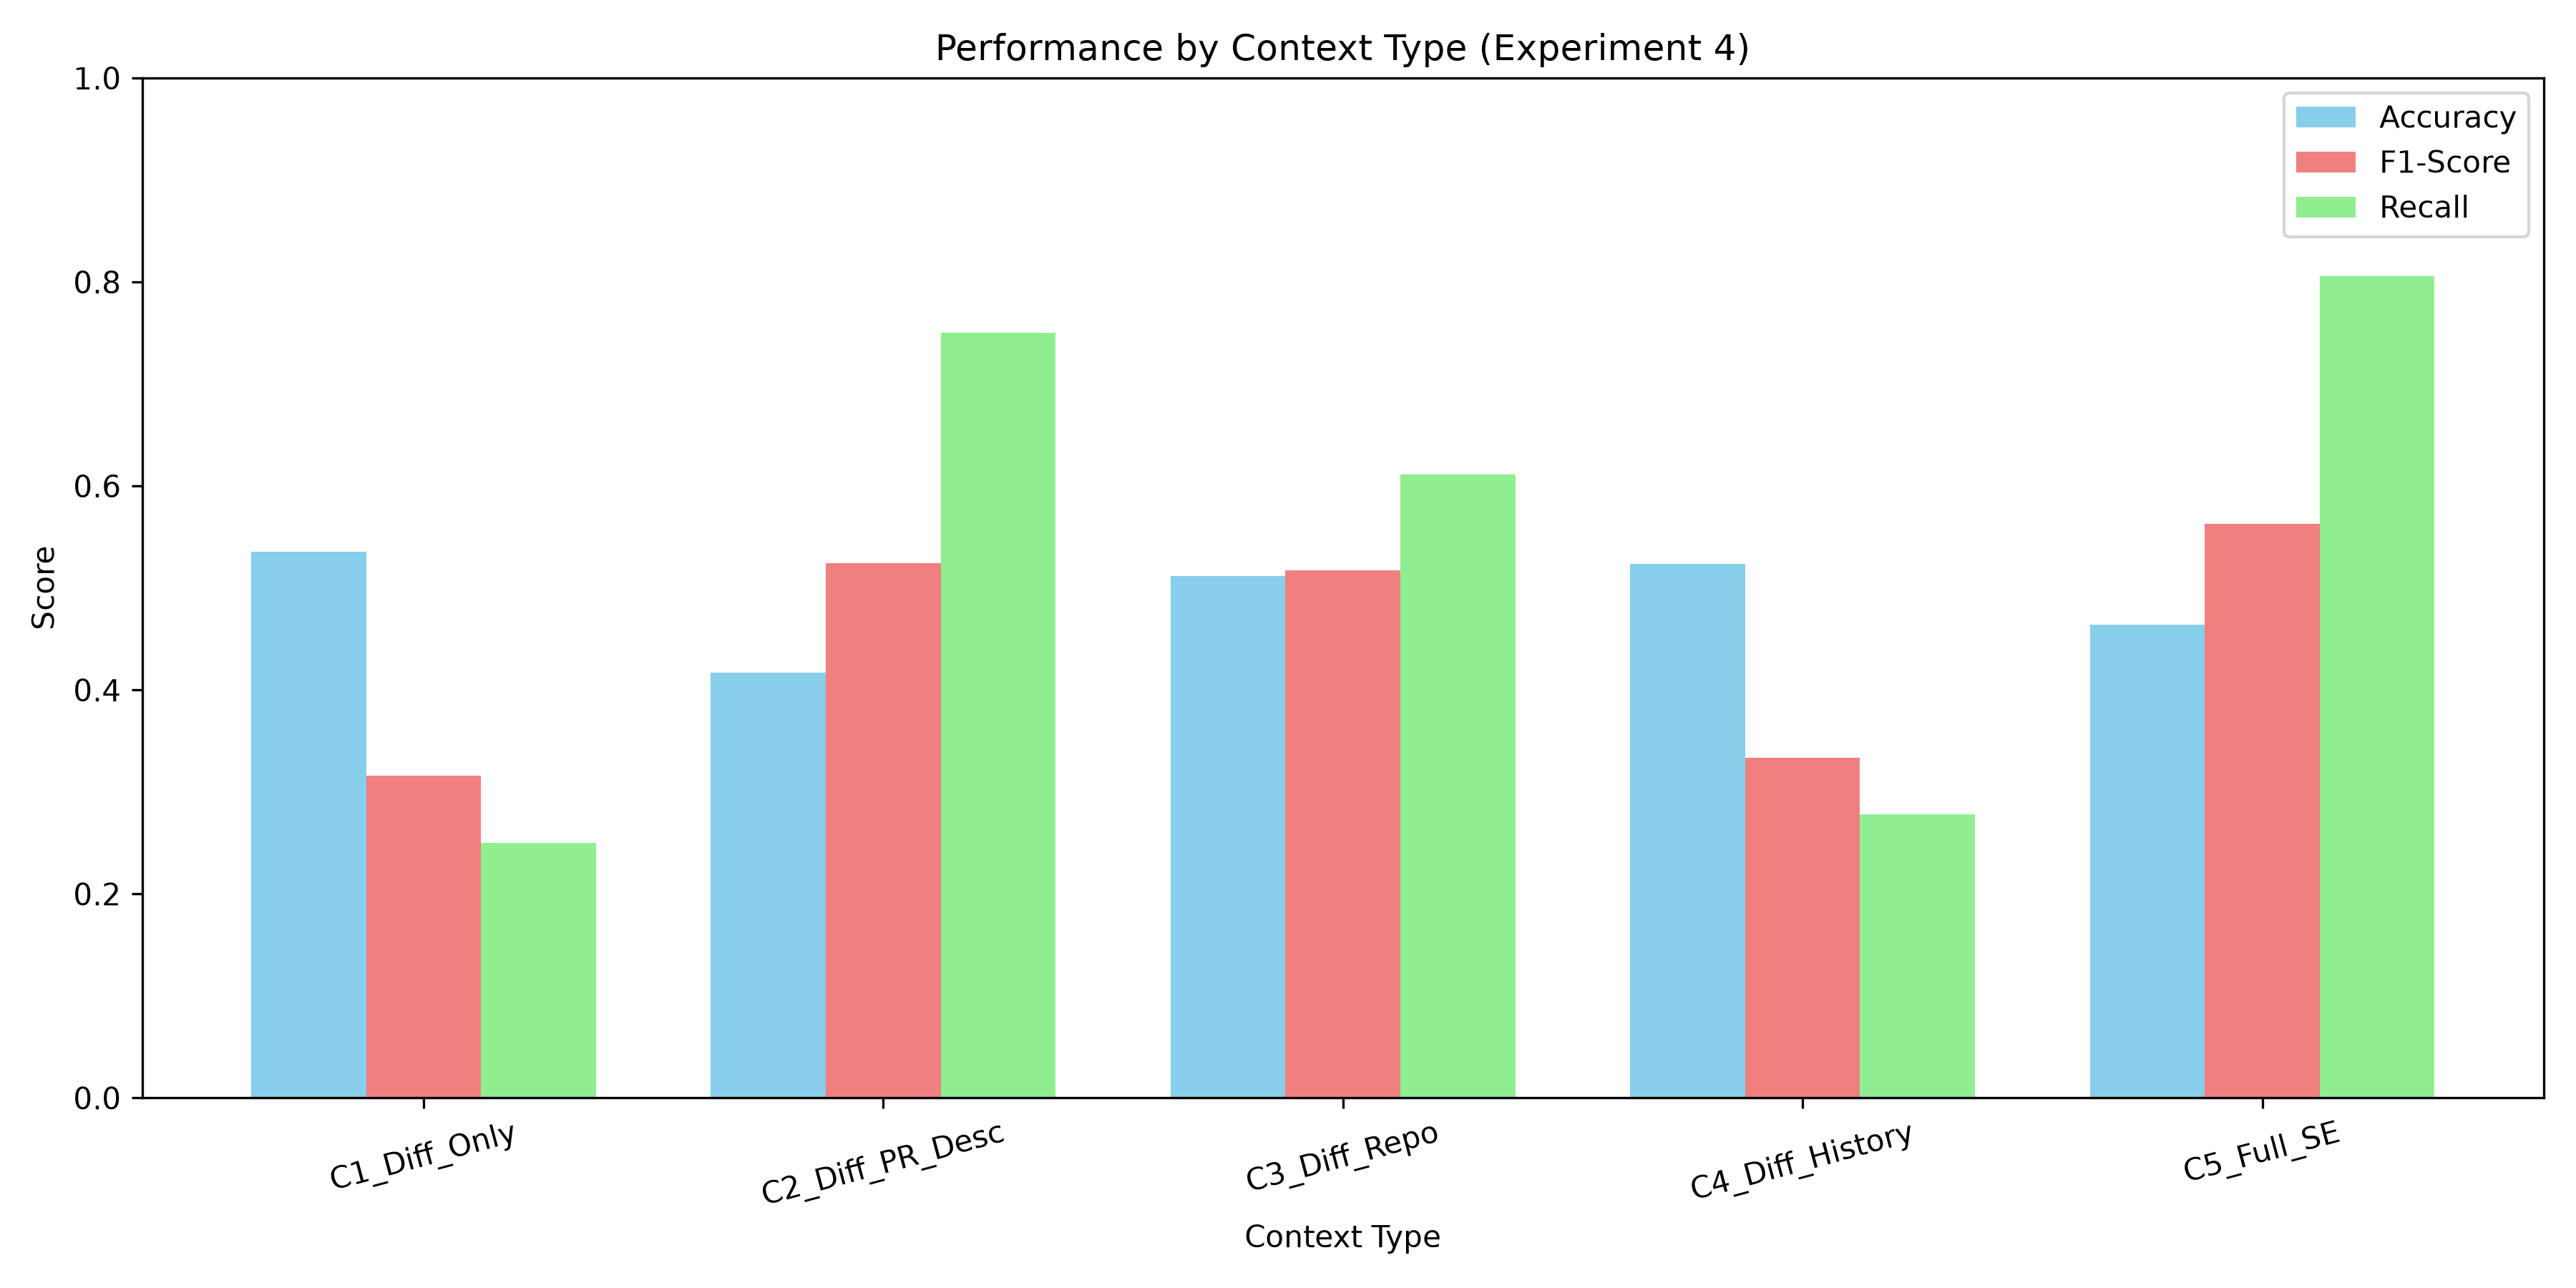
\includegraphics[width=0.8\textwidth]{exp4_context_comparison.png}
\caption{Performance comparison across different context types (C1-C5)}
\end{figure}

\begin{figure}[h]
\centering
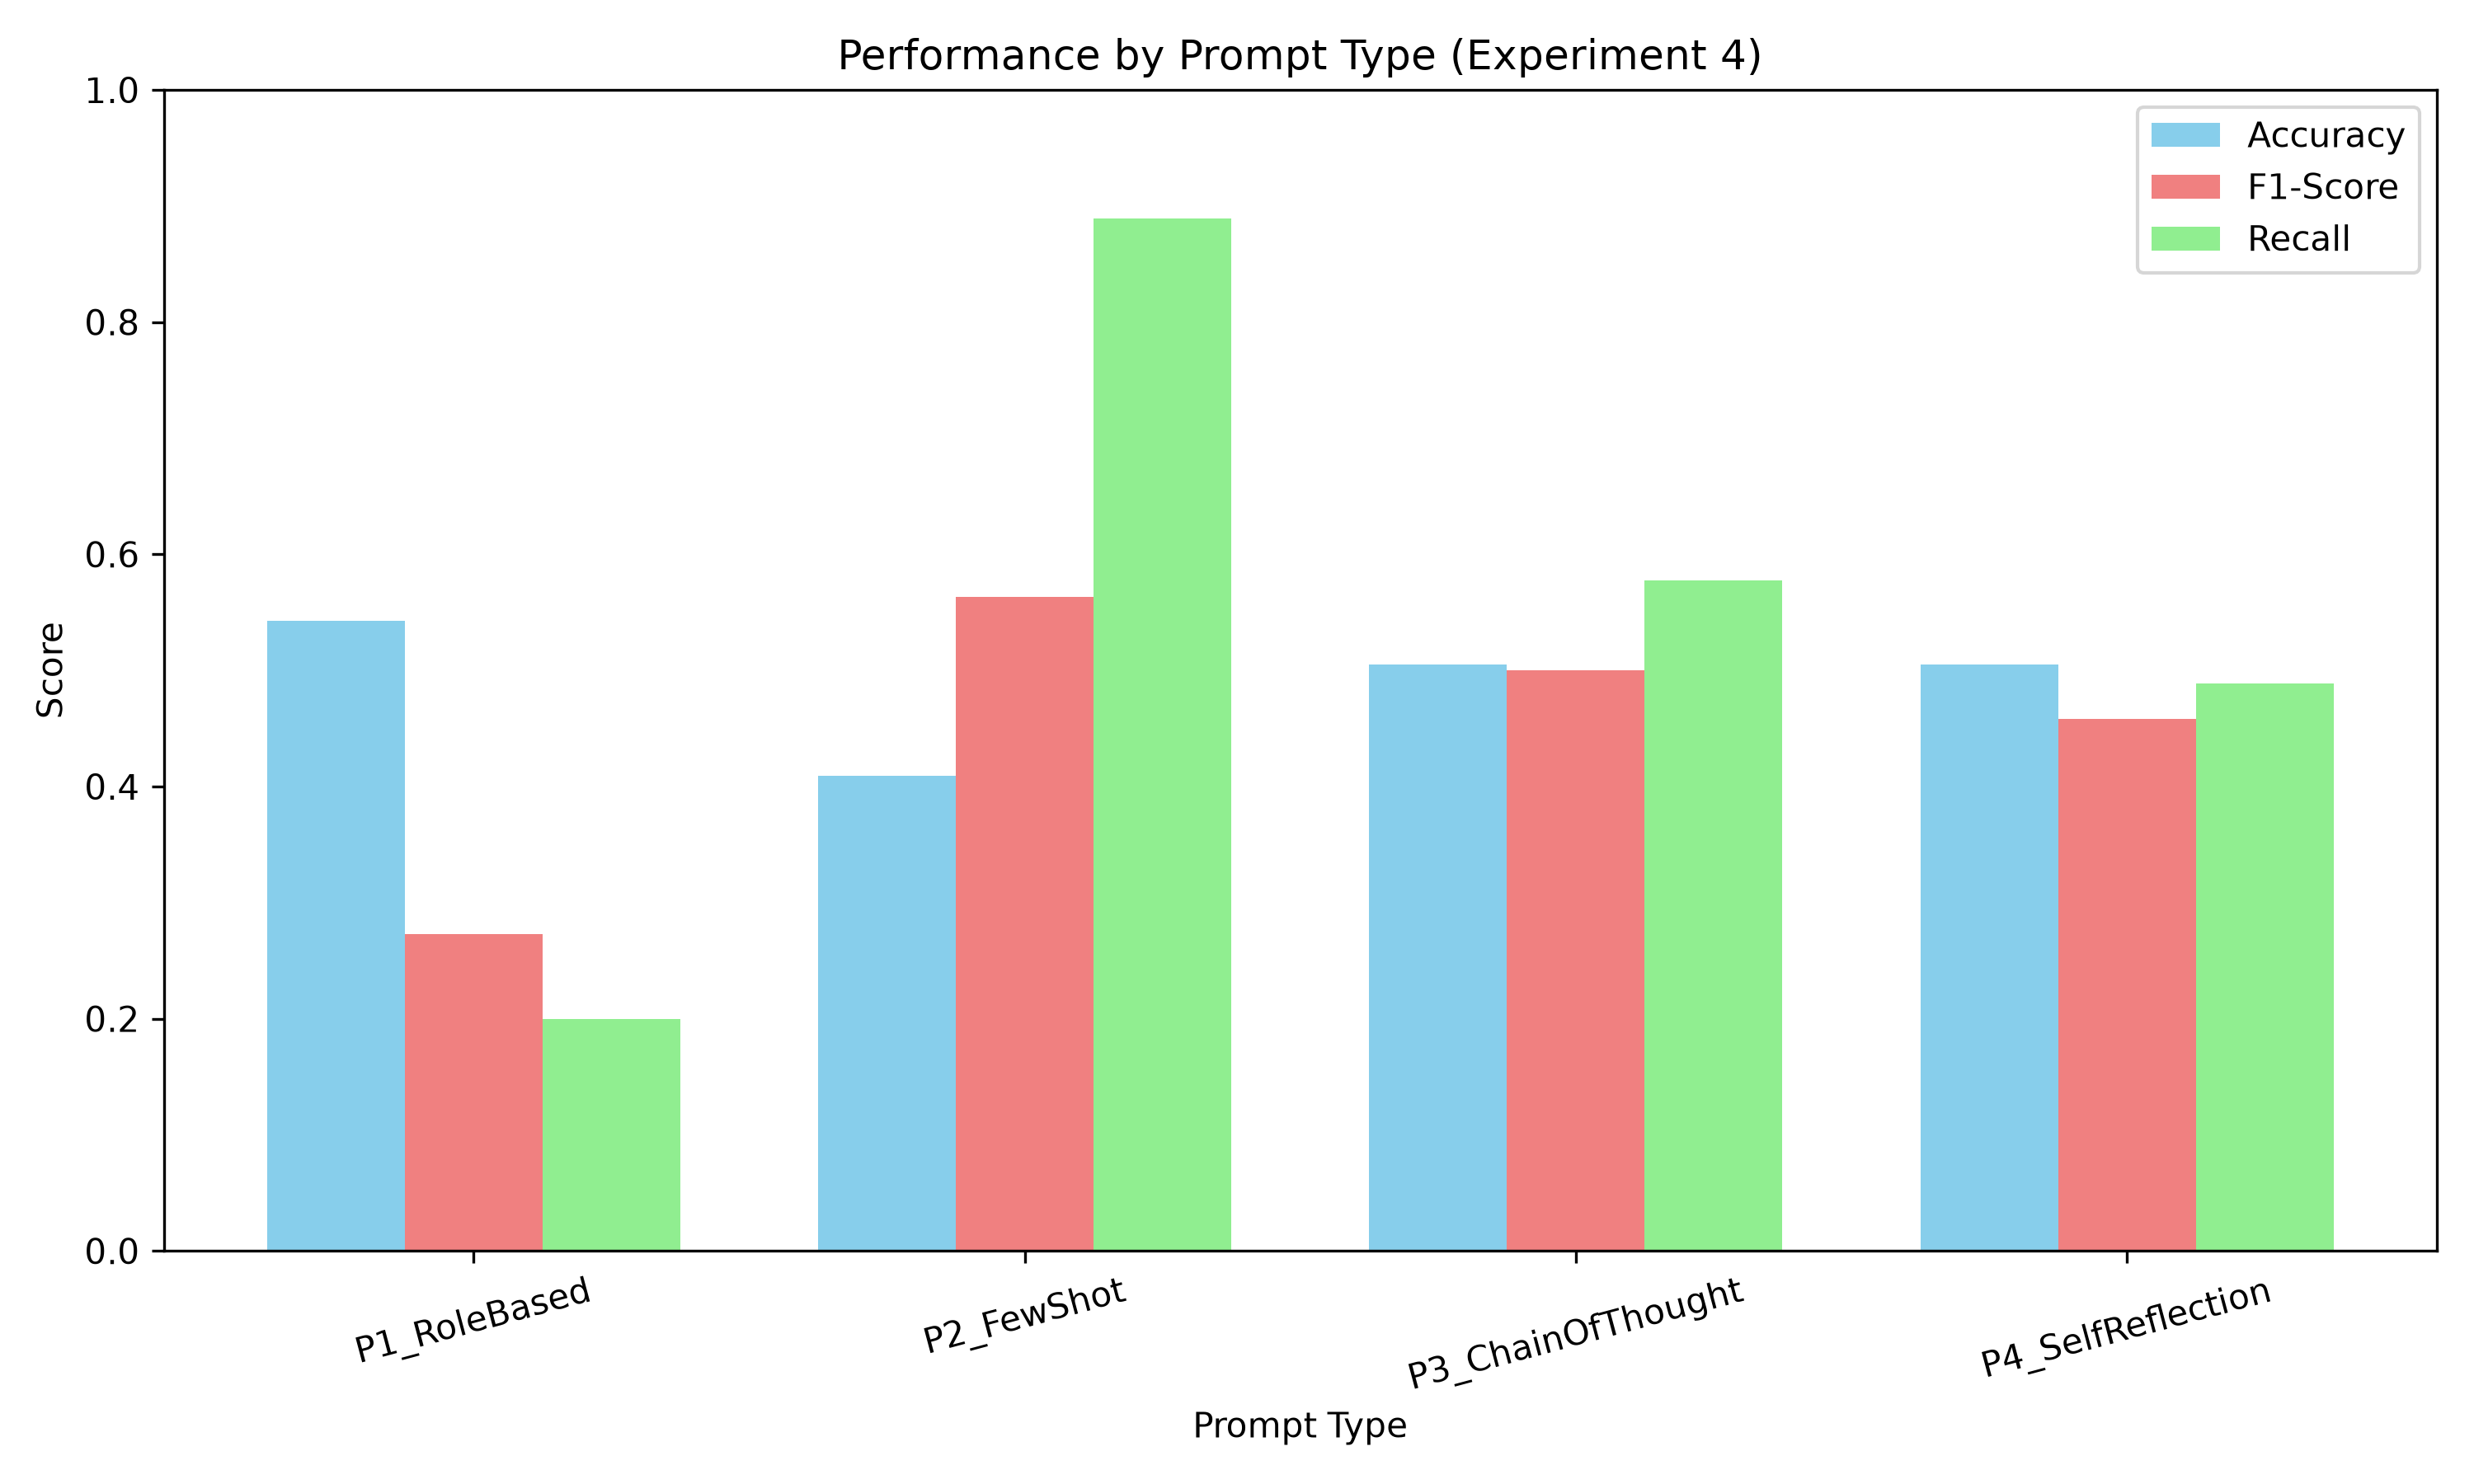
\includegraphics[width=0.8\textwidth]{exp4_prompt_comparison.png}
\caption{Performance comparison across different prompt optimization strategies (P1-P4)}
\end{figure}

\begin{figure}[h]
\centering
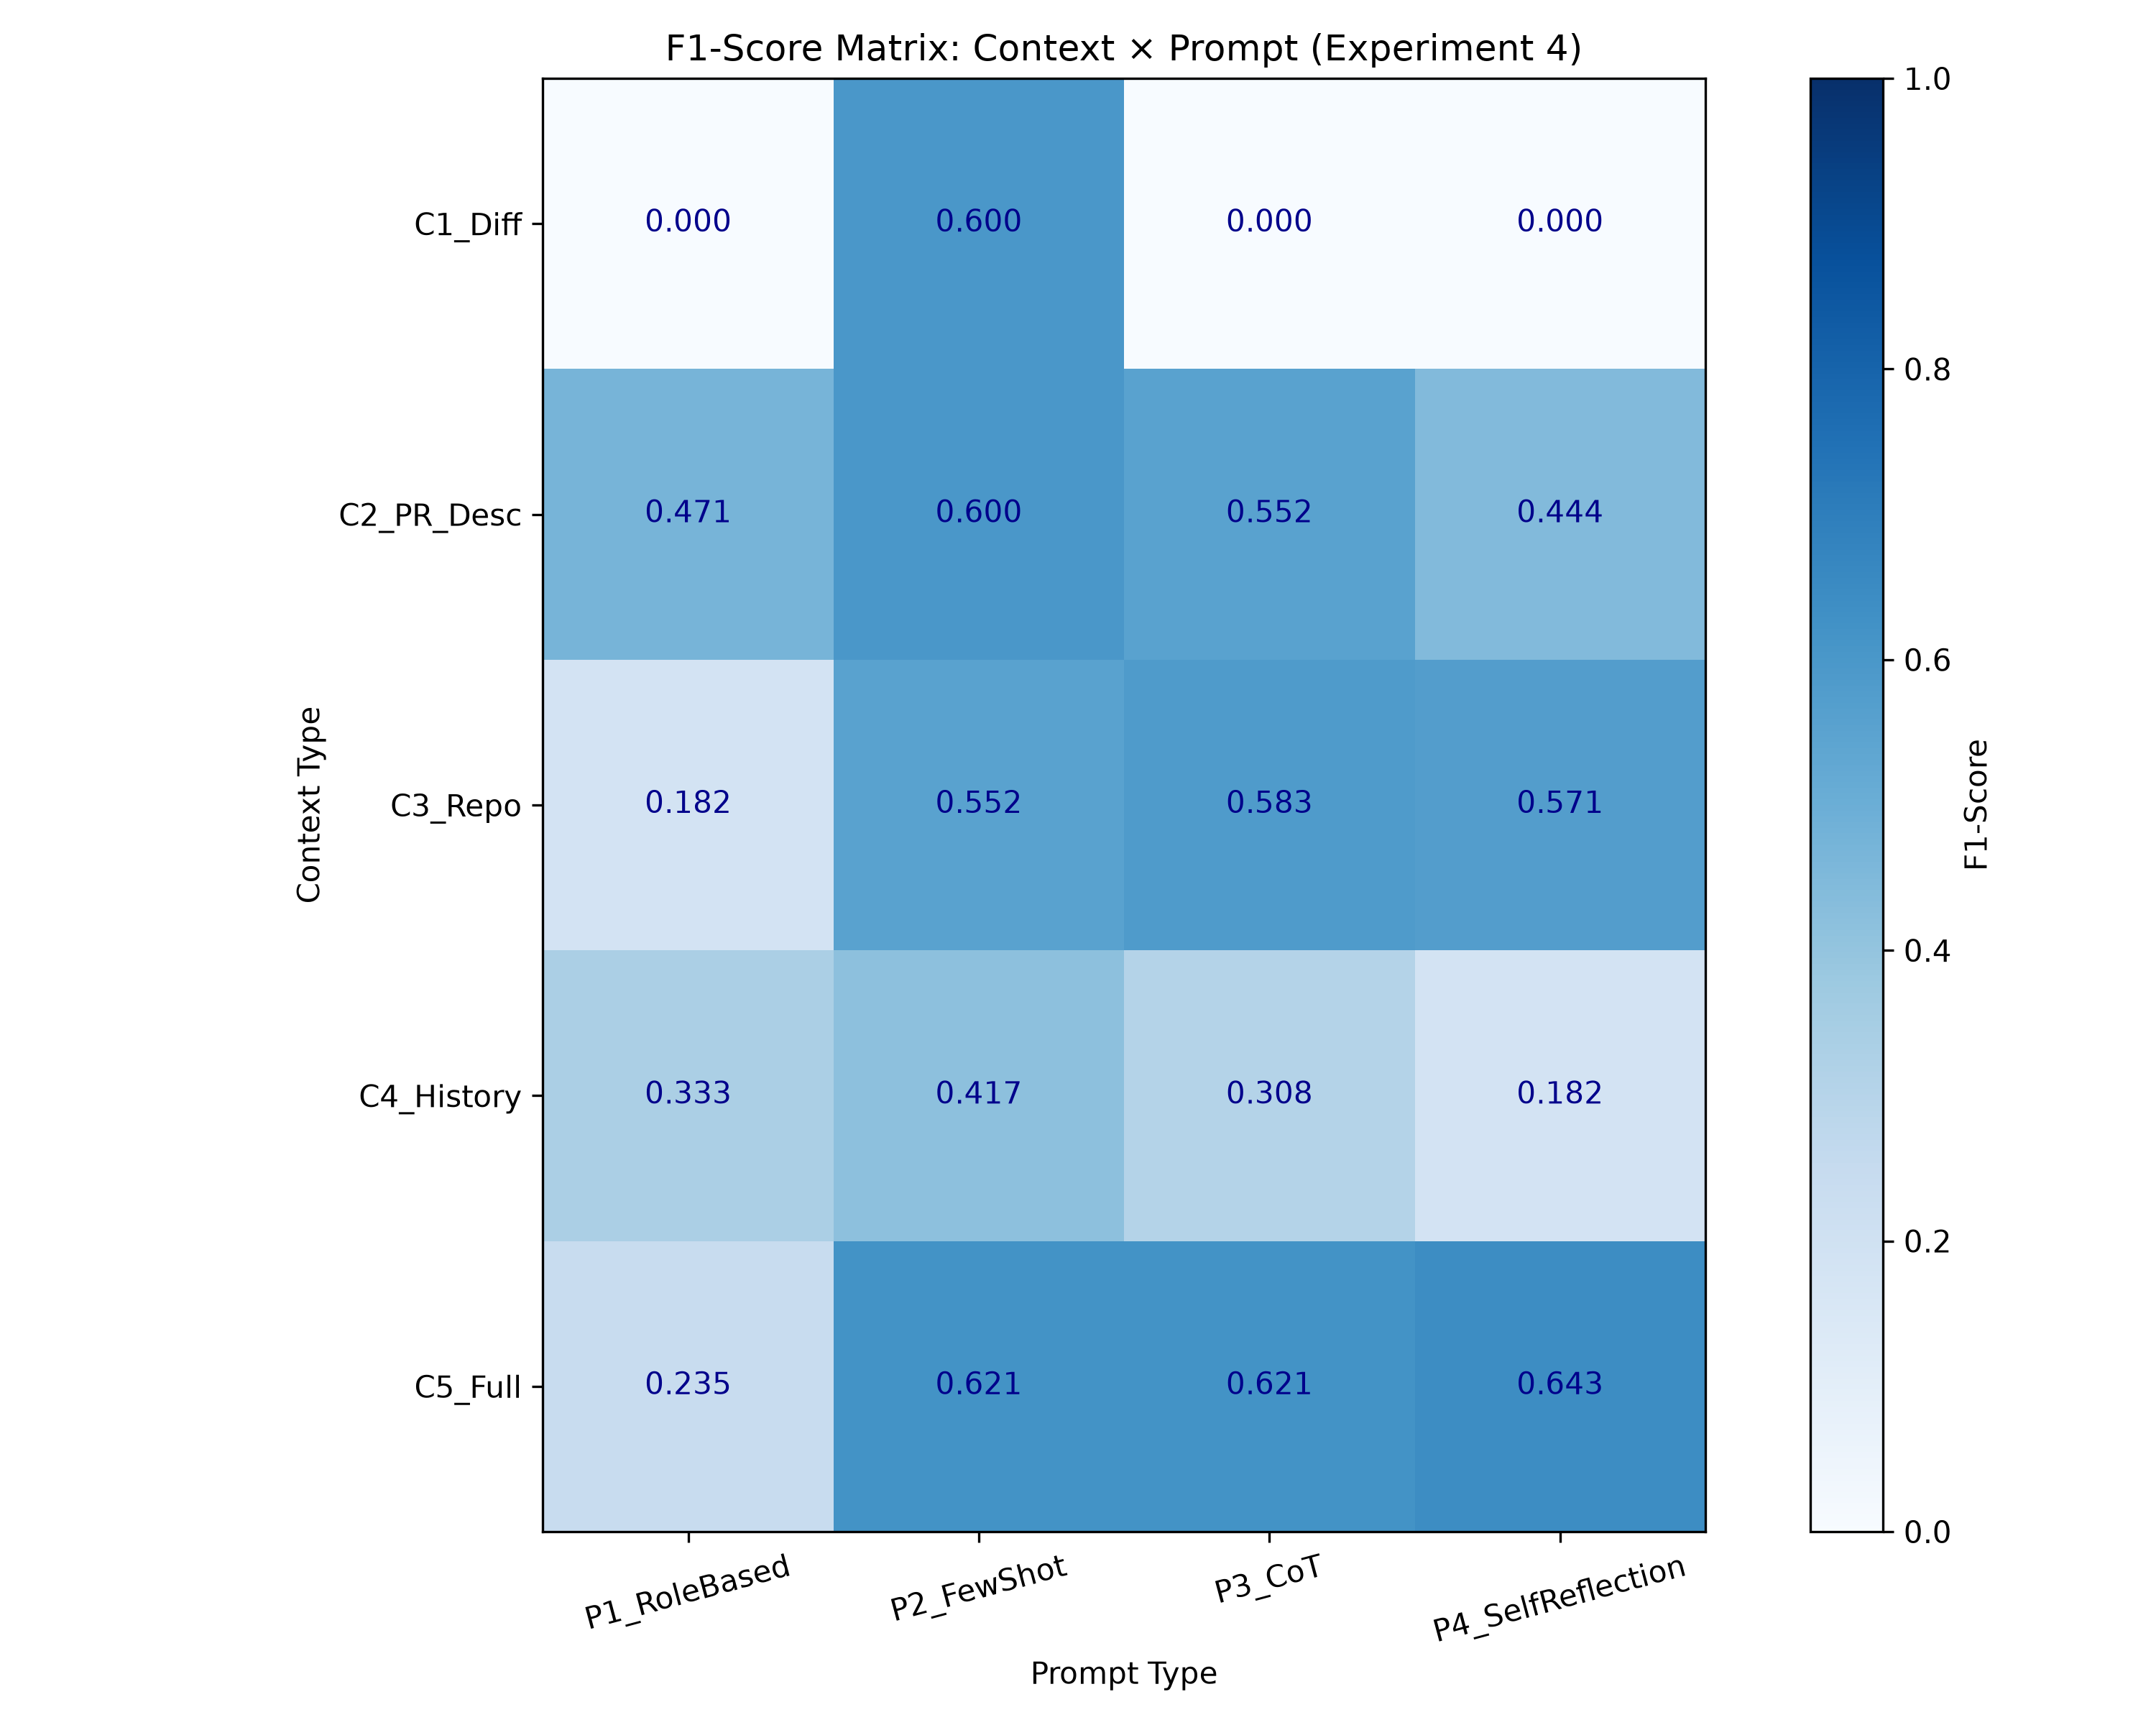
\includegraphics[width=0.8\textwidth]{exp4_f1_heatmap.png}
\caption{F1-Score matrix showing performance of each context-prompt combination}
\end{figure}

Comparison with Experiment 3 (Human-Written Code):
Metric                 Exp 3 (Human)   Exp 4 (AI)     Change
Best Accuracy          58.6\%          53.6\%         -5.0\%
Best F1-Score          66.2\%          56.3\%         -9.9\%
Best Recall            78.3\%          80.6\%         +2.3\%
Avg Latency            6.08s           7.06s          +0.98s
Best Context           C3\_Diff\_Commit C5\_Full\_SE   Richer context needed
Best Prompt            P1/P2\_Zero/Few  P4\_SelfRefl.  Reflection helps for AI

Key insight: AI-generated code requires richer context (C5) and self-reflection prompting (P4) to achieve comparable performance. The drop in F1 (9.9\%) shows that reviewing AI code is inherently more challenging.
}

%========================
% Context Examples
%========================

\section*{Context Examples}

\begin{itemize}
\item \textbf{C1\_Diff\_Only:} Only the code diff showing changes between versions.
\item \textbf{C2\_Diff\_PR\_Description:} Diff + PR title + author + PR description + commit messages.
\item \textbf{C3\_Diff\_Repo\_Metrics:} Diff + changed files count, additions/deletions, labels, commit messages.
\item \textbf{C4\_Diff\_Review\_History:} Diff + existing reviews and inline comments from previous reviewers.
\item \textbf{C5\_Full\_SE\_Context:} Complete context: diff + PR description + metrics + labels + commit messages + historical reviews + comments.
\end{itemize}

%========================
% Prompt Examples
%========================

\section*{Prompt Examples}

\begin{itemize}
\item \textbf{P1\_RoleBased:} "You are a Senior Staff Software Engineer inspecting Pull Requests containing AI-generated code. AI-generated code often looks plausible on the surface but can contain subtle logic errors, missing edge cases, or poor integration with existing repository structures. Perform a rigorous code review. Determine if this PR should be MERGED or REJECTED."

\item \textbf{P2\_FewShot:} "Example 1: [diff] → MERGE. Feedback: Good safeguard added against NoneType. Example 2: [diff] → REJECT. Feedback: Missing error handling. Now review this PR."

\item \textbf{P3\_ChainOfThought:} "Systematically analyze this AI-generated code step-by-step: (1) Intent \& Correctness, (2) Repository Consistency, (3) Edge Cases \& Security, (4) Final Output."

\item \textbf{P4\_SelfReflection:} "Phase 1: Formulate initial decision and review comments. Phase 2: Critically re-examine your Phase 1 decision. Did you overlook any context? Refine your reasoning. Provide final decision."
\end{itemize}

%========================
% Generated Review Comments Examples
%========================

\section*{Generated Review Comments Examples}

\textbf{PR \#327432 (C1\_Diff\_Only, P1\_RoleBased):}
"The provided code diff is empty, which means there are no changes to review in this Pull Request (PR). This could indicate that either the PR was mistakenly created without any modifications or that the changes were made but not included in the diff for some reason." → REJECT

\textbf{PR \#327432 (C1\_Diff\_Only, P2\_FewShot):}
"The PR adds a safeguard to handle NoneType elements in the sequence, which can prevent potential AttributeError when trying to access the 'price' attribute of an item that is None. This is a good practice and should be merged." → MERGE

%========================
% Problems Encountered
%========================

\experimentproblems{
- Limited dataset size for AI-generated PRs (only 21 PRs × 5 contexts × 4 prompts = 420 evaluations).
- Local Qwen model latency increased to 7.06 seconds per inference (vs 6.08s in Exp 3).
- Role-based prompting (P1) performed poorly for AI code (F1 = 27.3\%) - better to use Self-Reflection (P4).
- Self-reflection prompts sometimes produced contradictory Phase 1 vs Phase 2 answers - manually resolved conflicts.
- BLEU/ROUGE scores again registered 0.0 due to formatting mismatches between generated and reference texts.
- Some AI-generated PRs had empty diffs, causing the LLM to output irrelevant reviews.
}

%========================
% Reflections
%========================

\experimentexperience{
- Repository-level context (C5) improves code review performance for AI-generated code because AI lacks awareness of project-specific patterns and conventions. Human reviewers have this context implicitly; AI reviewers need it explicitly.

- Self-reflection prompting (P4) works best for AI-generated code because it forces the model to critically evaluate its own analysis, catching hallucinations and overlooked edge cases common in AI code.

- Prompt optimization addresses reasoning quality (how the model thinks); context augmentation addresses information completeness (what the model knows). Both are needed for AI code review.

- Different prompts work for different tasks. Role-based prompts work better for human code; self-reflection is specifically beneficial for AI code where hallucinations are more common.

- Future improvements could include: (a) retrieval-augmented generation (RAG) for better context retrieval, (b) multi-agent review systems where different agents specialize in different aspects, (c) fine-tuning on code review data, (d) integrating static analysis tools to verify AI-generated code.
}

%========================
% Instructor Comments
%========================

\teachercomment

\end{document}